\section{DevOps}
\label{sec:devops}

O termo DevOps tem sido usado com frequência em diversas esferas do
desenvolvimento de software da atualidade, mas por ser um conceito recente
(2008), muita cunfusão ainda é gerada ao tentar definir e trabalhar com DevOps.~\cite{adambertram:2016}
A palavra DevOps vem de duas palavras em inglês, \textit{development} e \textit{operations}
(desenvolvimento e operações) e de maneira geral é a cultura, movimento
ou conjunto de práticas que incentiva a comunicação, a colaboração e a integração de
desenvolvedores de software e outros profissionais de TI. Além das práticas 
também engloba ferramentas e técnicas que que automatizam o processo de entrega
de software e as mudanças de infraestrutura~\cite{loukides2012devops}~\cite{erich2014mapping}.

Muitas vezes o termo é confundido com uma nova responsabilidade, ou cargo
dentro de uma empresa que desenvolve software, e por mais que seja possível
ter profissionais que tenham proficiência nas ferramentas relacionadas a
DevOps, o ideal, como dito anteriormente, é ter uma melhor comunicação,
colaboração e integração entre os times já existentes. As ferramentas
relacionadas à DevOps facilitam esses aspectos, mas o diferencial é a
mudança no processo de desenvolvimento para absorver essas melhorias.~\cite{adambertram:2016}

A ferramenta proposta por esse Trabalho de Conclusão de Curso entra na categoria
de ferramentas DevOps que agilizam a configuração de ambientes, podendo ser ambientes
de produção ou desenvolvimento.

%TODO: parece está faltando mais alguma coisa de DevOps, não sei o q =p

\subsection{Metodologia Ágil}

A metodologia ágil surgiu como uma resposta às maneiras tradicionais de desenvolvimento
de software considerando uma nova abordagem com relação a práticas, organização,
documentação e foco no desenvolvimento em si.~\cite{agilemetorg:2016}

A maneira mais popular de se introduzir agilidade a um projeto é o Scrum. O Scrum
foca principalmente em retorno empírico de métricas, auto gerenciamento de
equipes e esforço para construir produtos testados de maneira 
satisfatória.~\cite{agilemetorg:2016}

\subsubsection{Metodologia Iterativa}

Diferentemente da metodologia de Cascata, por exemplo, o Scrum implementa uma
abordagem iterativa e incremental, podendo assim desenvolver incrementos de
maior valor pro cliente mais cedo, e assim tendo \textit{feedback} para correções
mais frequentes. A figura~\ref{fig:iterative} mostra um exemplo dessas
Iterações.~\cite{scrumreference:2016}

\begin{figure}[H]
  \centering
  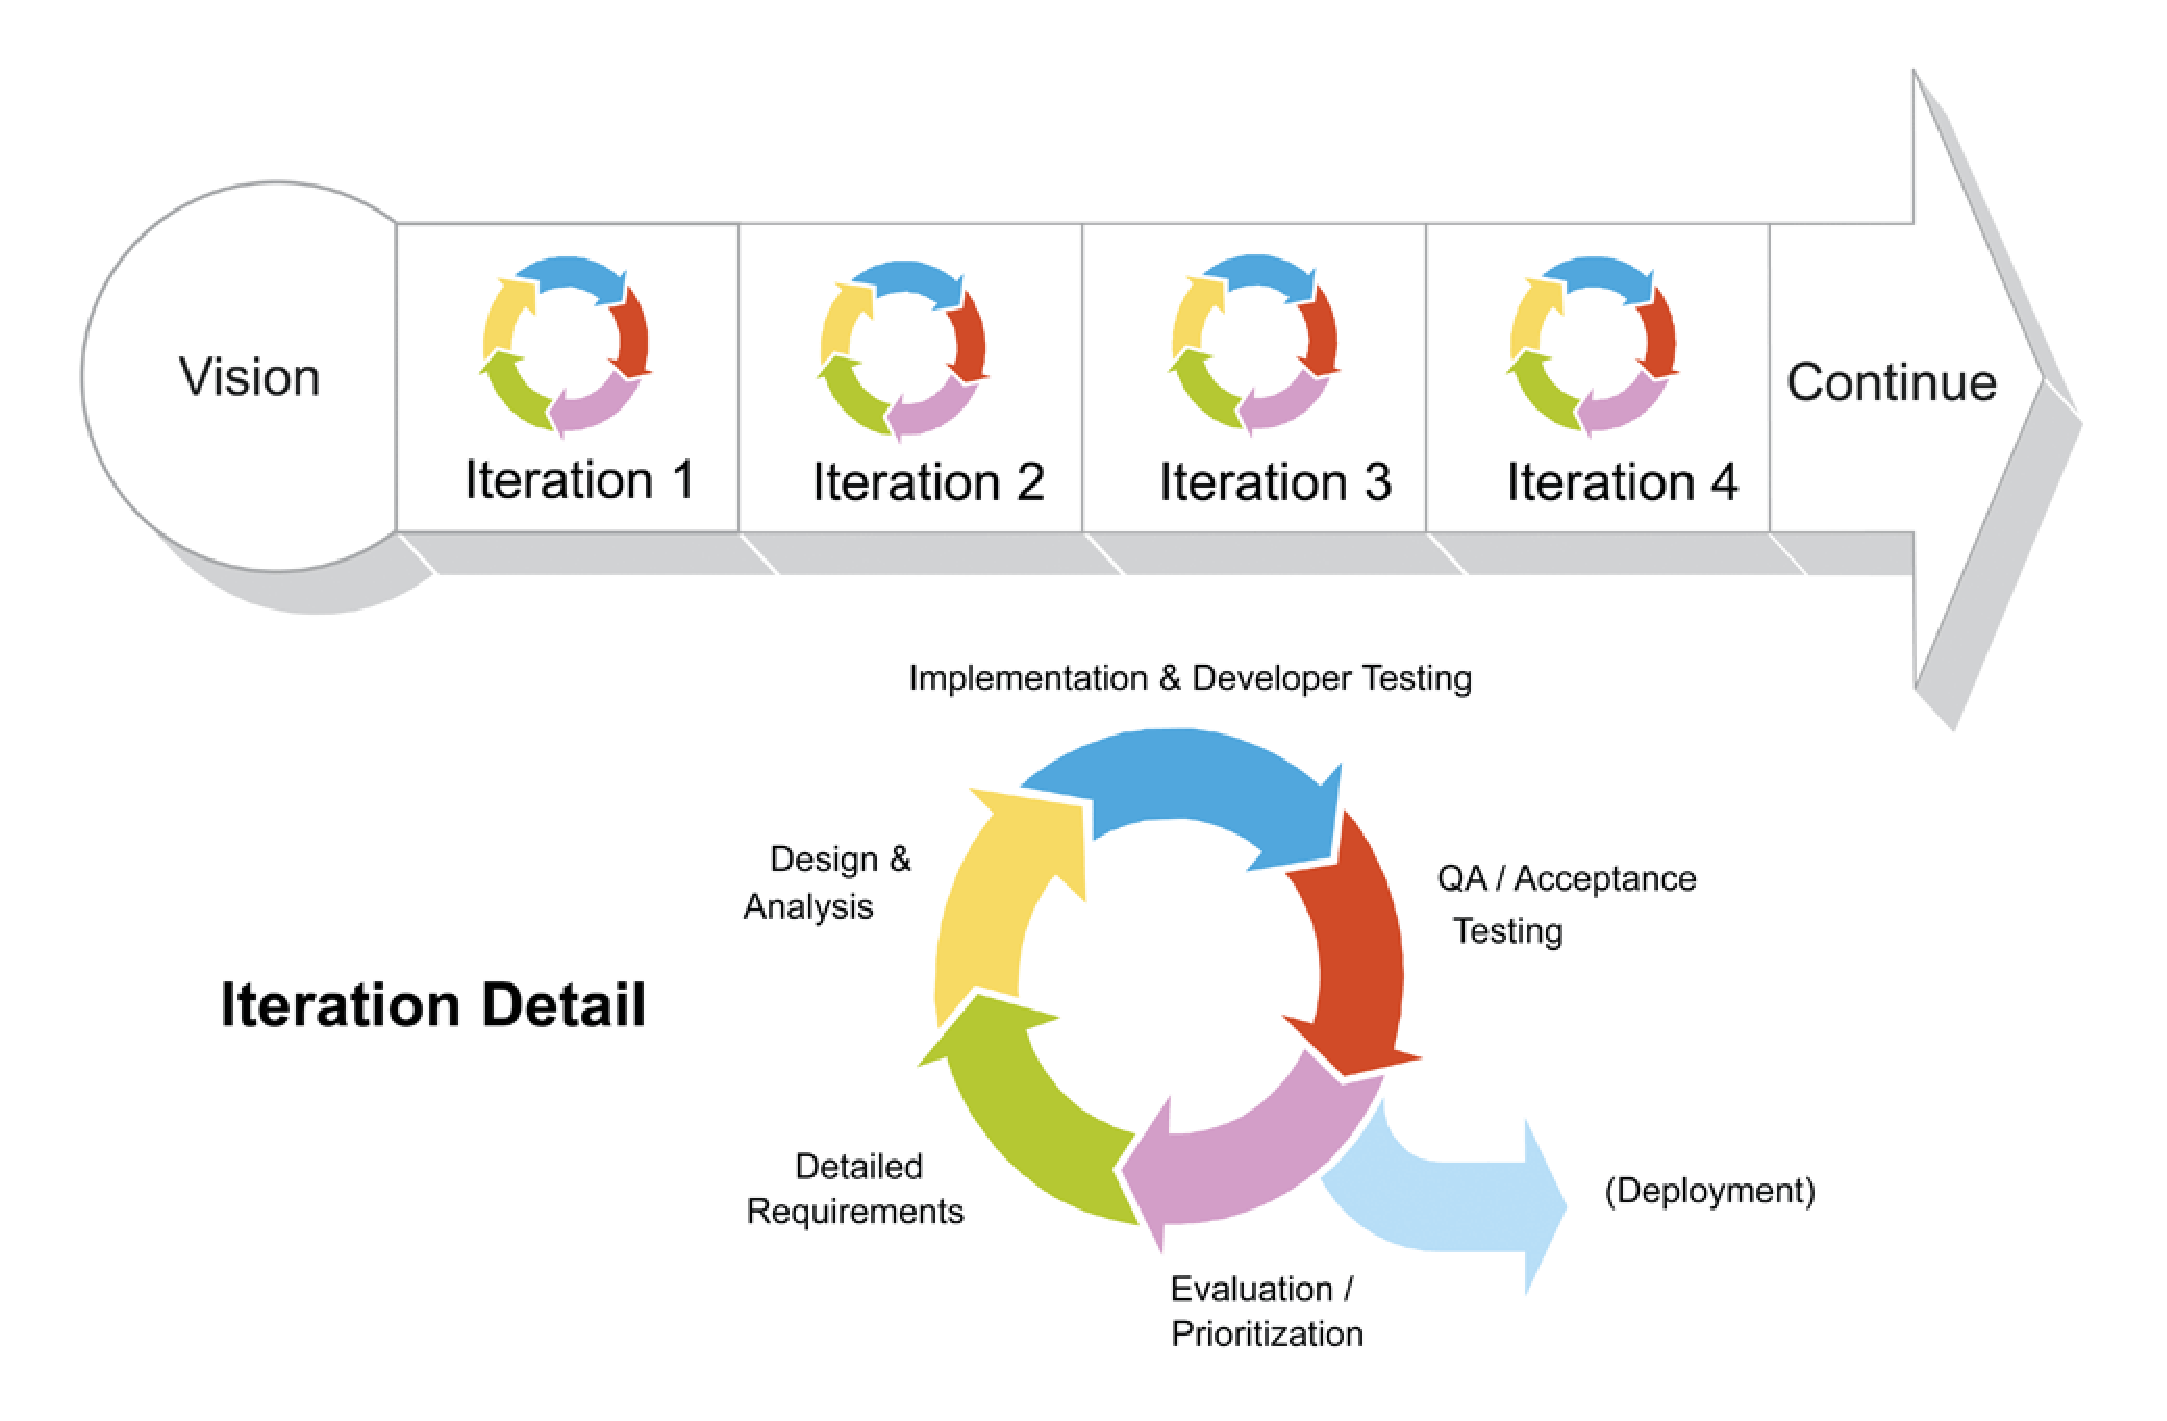
\includegraphics[width=0.8\textwidth]{figuras/iterative.eps}
  \caption{Iterações do Scrum}
  \label{fig:iterative}
\end{figure}

\subsubsection{Papéis}

Outros tipos de metodologias ágeis possuem algumas outras características, outros
papéis, e conjuntos diferentes de práticas. O Scrum é o mais popular por sua
simplicidade~\cite{ilieva2004analyses}. Um dos pontos importantes dessa
simplicidade é a existência de somente três papéis oficiais da metodologia. O 
PO (\textit{Product Owner}, dono do produto) que é responsável por sempre dar
retorno referentes às entregas frequentes do time, pela visão do produto,
e decisões de entregas. O time de desenvolvimento Scrum, que inclui profissionais
com habilidades não tradicionais de desenvolvedores, como gerenciamento de
infraestrutura, análise de negócio ou expertize do domínio, além de
desenvolvedores clássicos. E por fim o ScrumMaster que tem responsabilidades
relacionadas à facilitar o processo do Scrum, criar um ambiente que propicie
auto organização, proteger o time de interferências que atrapalhem o seu foco e
manter as práticas ágeis e do Scrum dentro dos
padrões~\cite{scrumreference:2016}.

\subsubsection{Scrum Meeting}

Já que o Scrum prega a maior comunicação entre a equipe, entre si e com o cliente,
diversas reuniões são previstas na metodologia. A figura~\ref{fig:scrum_flow}
mostra o fluxo dessas reuniões.

\begin{figure}[H]
  \centering
  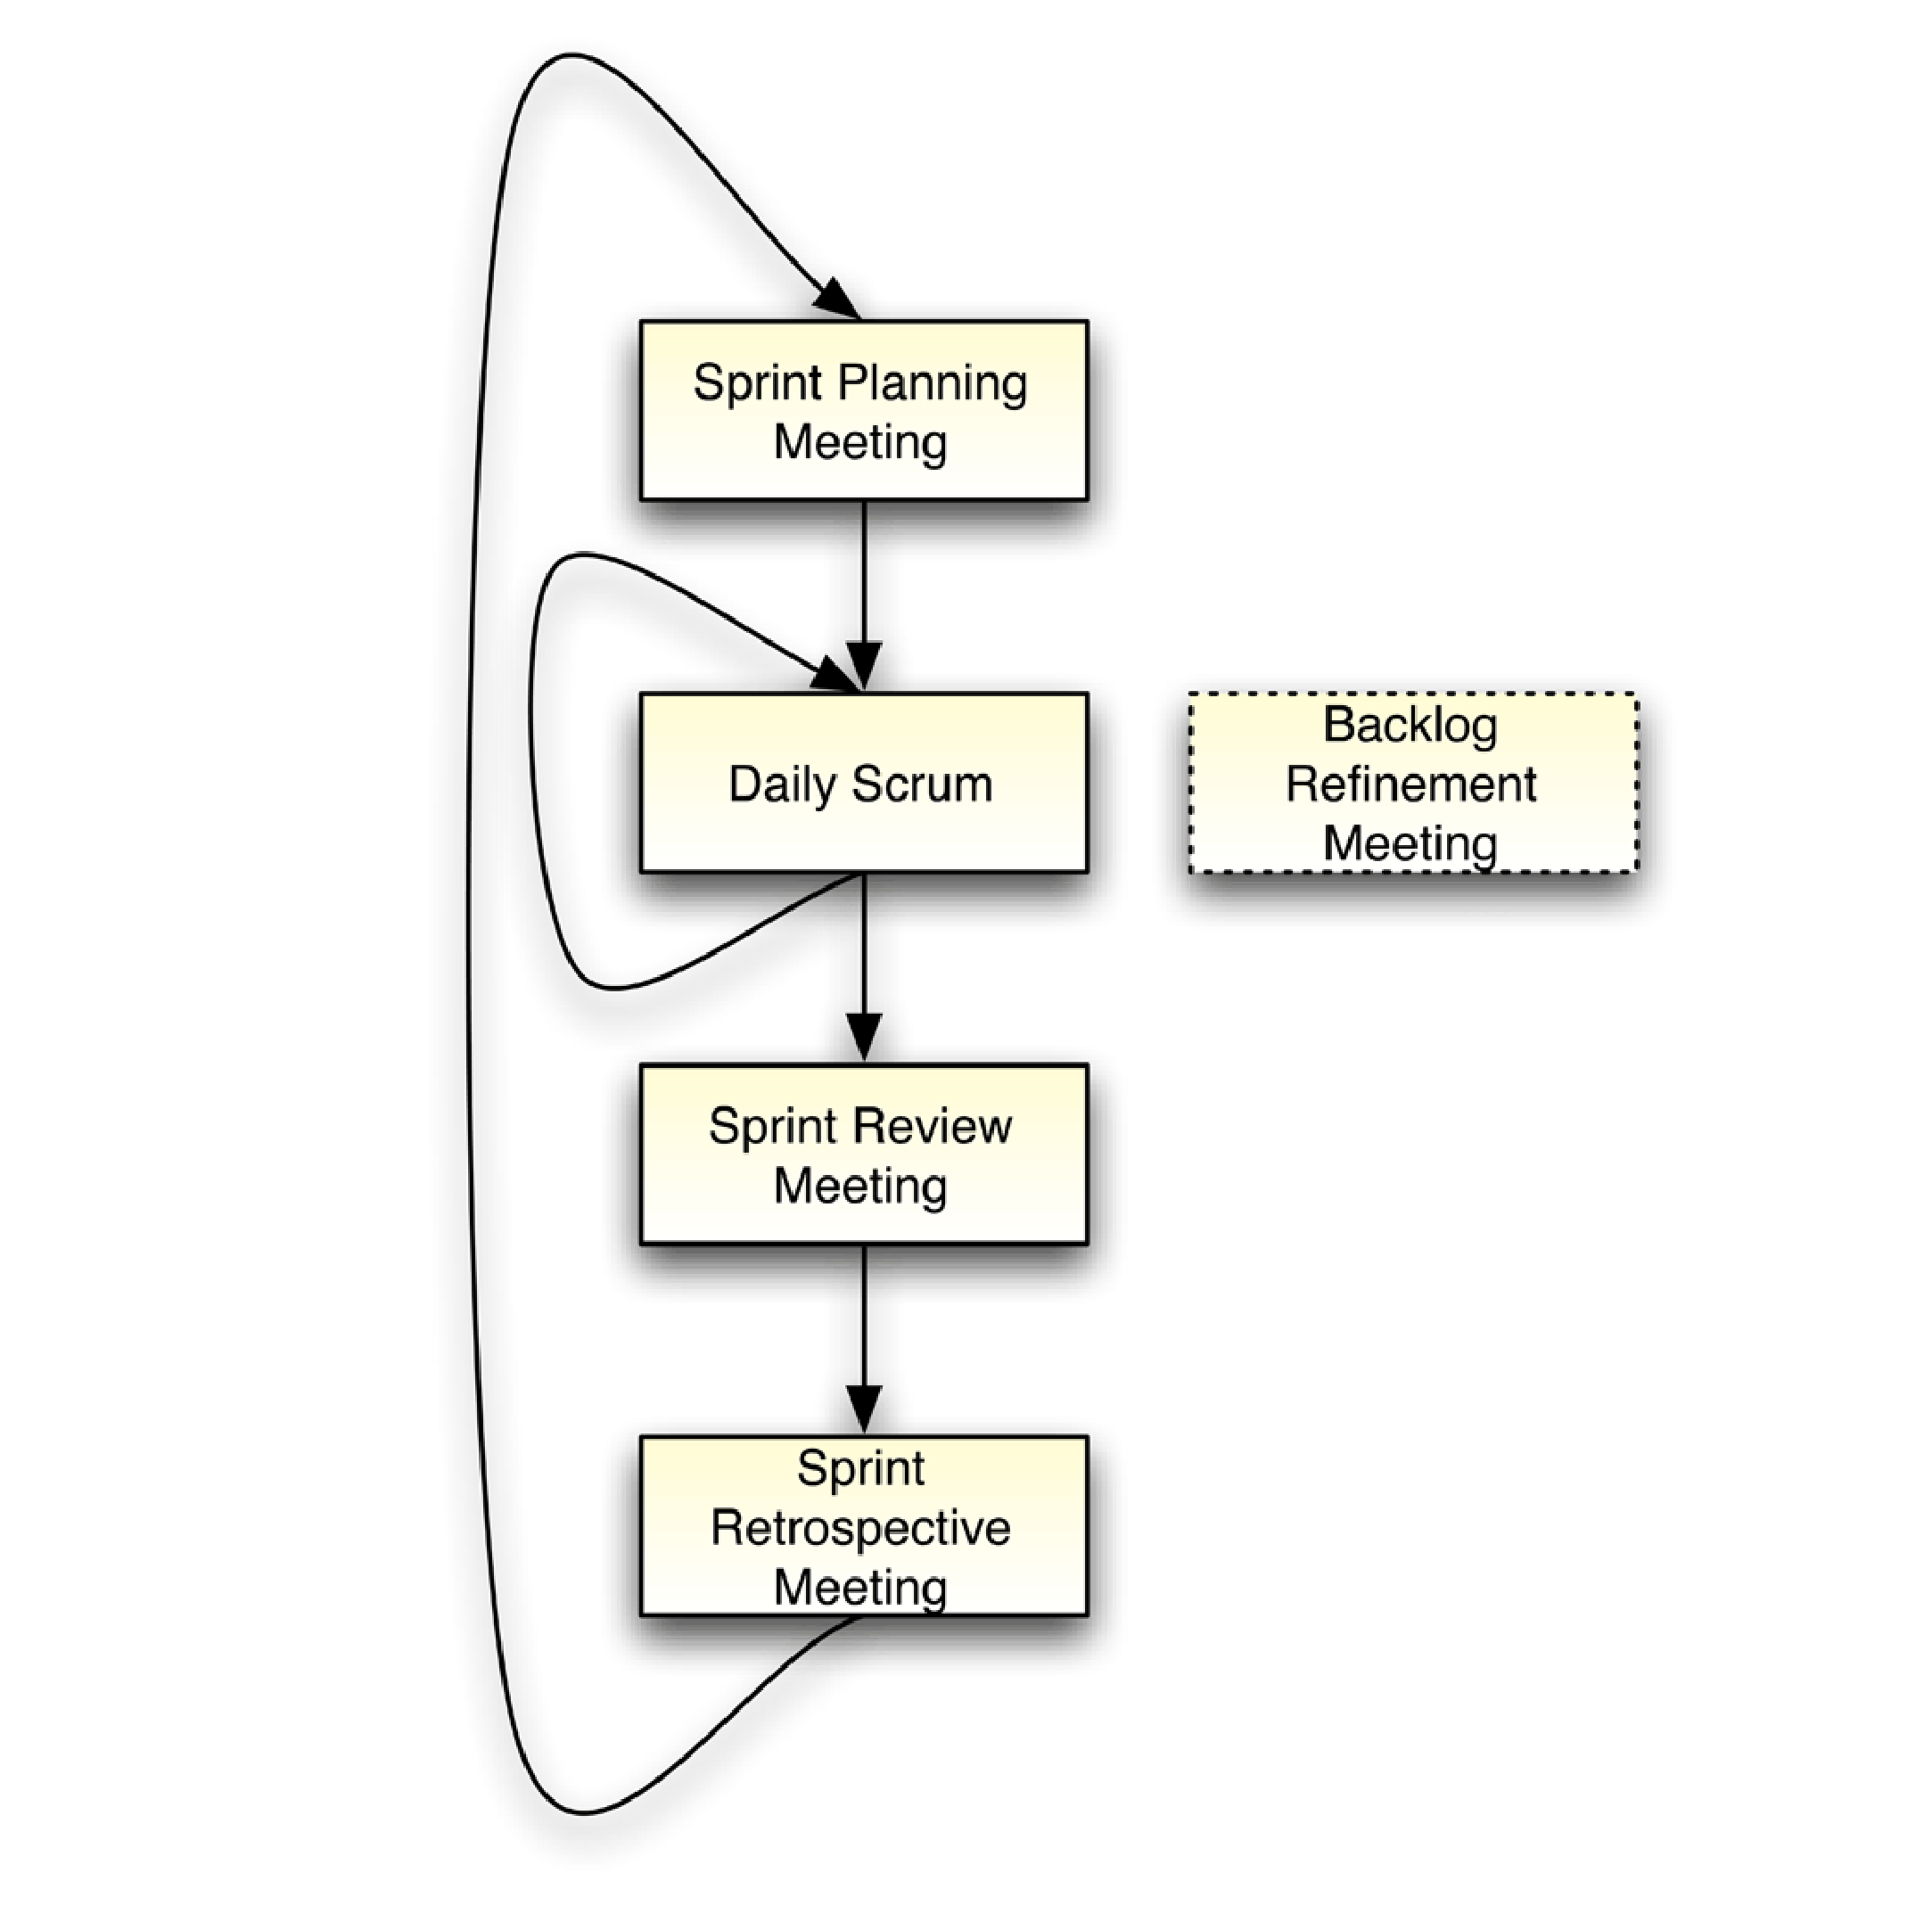
\includegraphics[width=0.8\textwidth]{figuras/scrum_flow.eps}
  \caption{Fluxo Scrum}
  \label{fig:scrum_flow}
\end{figure}

\subsubsection{Prática Relacionada - XP}

Um exemplo de metodologia de desenvolvimento ágil muitas vezes utilizado em
conjunto com o Scrum é a \textit{eXtreme Programming} (XP). O ScrumMaster pode
incentivar o time a utilizar práticas do XP, como integração contínua, 
desenvolvimento orientado a testes, pareamento, dentre outras.

\subsection{Metodologia Ágil e DevOps}

Com a popularização da metodologia de desenvolvimento Ágil, que tem, dentre outros
objetivos, o de entregar com maior frequência, e melhorar a comunicação entre os
times, é simples fazer a relação de DevOps com esse tipo de desenvolvimento.
DevOps nada mais é do que a implementação de conceitos e mudanças organizacionais
e culturais provenientes do pensamento Ágil \cite{scott2014}.

DevOps tenta alcançar entregas mais frequentes ao preparar um ambiente que facilite,
automatize e integre vários dos processos que antes seriam manuais, e mais
suscetíveis à falhas e atrasos, o que não é possível sem uma equipe integrada
nesse ambiente. Dessa forma, o conceito de entrega contínua e de integração
contínua estão fortemente relacionados à DevOps.~\cite{adambertram:2016}

%TODO: acho melhor incluir integração contínua e entrega contínua dentro desse tópico e correlacionar com devops e agil

\subsection{Integração Contínua}

Integração contínua é a prática de integrar diversas partes de um software
desenvolvido em diversas frentes, de maneira periódica, ou a cada mudança.
Foi adotado como parte da \textit{extreme programming} (XP) que sugere integrar
partes do software mais de uma vez por dia \cite{fowler2006continuous}.

Mesmo que não se adote desenvolvimento orientado a teste (TDD - test driven 
development), uma funcionalidade só está pronta se estiver com seus testes 
implementados, levando em consideração metodologias de desenvolvimento Ágil. 
E dessa forma a integração contínua pode dar retorno com relação aos resultados
desses testes a todo momento que ocorrer uma nova integração do software.

\subsection{Entrega Contínua}

A Entrega Contínua é uma prática adotada pelos métodos ágeis que tem o objetivo
de preparar um \textit{software} para que ele seja passível de ser posto em produção a
qualquer momento~\cite{olausson:2016}. %TODO: melhorar a construção dessa frase.

A prática de Entrega Contínua  é frequentemente confundido com a Integração
Contínua. Existe uma relação de dependencia entre as duas práticas para
construir uma estrutura que possa sustentar a entrega contínua de um
\textit{software}.~\citeonline{olausson:2016} resume os dois em:

\begin{itemize}
  \item \textbf{Integração Contínua}: é voltada para estabelecer uma rápida
    validação da fase de desenvolvimento;
  \item \textbf{Entrega Contínua}: é voltada para estabelecer uma cultura onde
    pode-se oferecer um recurso ou \textit{feature} para o cliente a qualquer
    momento.
\end{itemize}

